\let\negmedspace\undefined
\let\negthickspace\undefined
\documentclass[journal]{IEEEtran}
\usepackage[a5paper, margin=10mm, onecolumn]{geometry}
%\usepackage{lmodern} % Ensure lmodern is loaded for pdflatex
\usepackage{tfrupee} % Include tfrupee package

\setlength{\headheight}{1cm} % Set the height of the header box
\setlength{\headsep}{0mm}     % Set the distance between the header box and the top of the text

\usepackage{gvv-book}
\usepackage{gvv}
\usepackage{algorithmicx} % Ensure algorithmicx is loaded explicitly
\usepackage{cite}
\usepackage{amsmath,amssymb,amsfonts,amsthm}
\usepackage{graphicx}
\usepackage{textcomp}
\usepackage{xcolor}
\usepackage{txfonts}
\usepackage{listings}
\usepackage{enumitem}
\usepackage{mathtools}
\usepackage{gensymb}
\usepackage{comment}
\usepackage[breaklinks=true]{hyperref}
\usepackage{tkz-euclide} 
\usepackage{listings}
% \usepackage{gvv}                                        
\def\inputGnumericTable{}                                 
\usepackage[latin1]{inputenc}                                
\usepackage{color}                                            
\usepackage{array}                                            
\usepackage{longtable}                                       
\usepackage{calc}                                             
\usepackage{multirow}                                         
\usepackage{hhline}                                           
\usepackage{ifthen}                                           
\usepackage{lscape}
\usepackage{algorithm}
\usepackage{algpseudocode}

\renewcommand{\thefigure}{\theenumi}
\renewcommand{\thetable}{\theenumi}
\setlength{\intextsep}{10pt} % Space between text and floats


\numberwithin{equation}{enumi}
\numberwithin{figure}{enumi}
\renewcommand{\thetable}{\theenumi}

% Marks the beginning of the document
\begin{document}
\bibliographystyle{IEEEtran}

\title{11.16.4.10}
\author{EE24BTECH11049 - Patnam Shariq Faraz Muhammed}

% \maketitle
% \newpage
% \bigskip
{\let\newpage\relax\maketitle}

\textbf{Question:}\\
The number lock of a suitcase has 4 wheels, each labeled with ten digits i.e., from 0 to 9. The lock opens with a sequence of four digits with no repeats. What is the probability of a person getting the right sequence to open the suitcase?\\

\textbf{Solution}\\
\begin{enumerate}
    \item \textbf{Total Number of Possible Sequences}\\
    Since each wheel has $10$ possible digits and no digit repeats in the sequence, implies that to get all the possible values of the sequence we need to arrange all the ten digits (0 to 9) in four places. (No repetitions)
    
    The total number of possible sequences is:
    \begin{align}
        \myvec{10 \\ 4} \times {4!} = 5040
    \end{align}
    or 
    \begin{align}
        10 \times 9 \times 8 \times 7 = 5040
    \end{align}
    This is because 
    \begin{itemize}
        \item The first wheel has 10 possible digits.
        \item The second wheel has nine possible digits (since one digit has already been used).
        \item The third wheel has 8 possible digits.
        \item The fourth wheel has 7 possible digits.
    \end{itemize}
    \item \textbf{Probability of Success}\\
    Out of all 5040 possibilities, only one sequence is right. The probability $p$ of guessing the right sequence 
    \begin{align}
        p &= \frac{1}{\text{Total number of possible sequences}}\\ &= \frac{1}{5040}\\ &= 0.000198
    \end{align}
    \newpage
    \item \textbf{Defining the Random Variable}\\
    We model this problem using Bernoulli random variables,\\
    Let $X$ be the random variable that represents the correct sequence of digits of the Wheel:
    \begin{align}
        X &= 1, \text{ If the sequence chosen is correct, \brak{\text{With probability }p = \frac{1}{5040}}}\\
        X &= 0, \text{ If the sequence chosen is incorrect, \brak{\text{With probability } 1 -p = \frac{5039}{5040}}}
    \end{align}
    \item \textbf{Probability Mass Function (PMF):}\\
    The PMF  of a Bernoulli random variable $X$ is given by:
    \begin{align}
	P\brak{X = x} = p^x\brak{1 - p}^{1 - x}, x \in \cbrak{0,1}
    \end{align}
    substituting $p = \frac{1}{5040}$,\\
    \begin{align}
     P\brak{X = 1} = 0.000198, P\brak{X = 0} = 0.999802
    \end{align}
    \begin{align}
    	P\brak{X = x} = \begin{cases}
    		0.000198, & x = 1 \\
    		0.999802, & x = 0 \\
    		0, & \text{otherwise}
    	\end{cases}
    \end{align}

    \item \textbf{Cumulative Distribution function (CDF):}\\
    The CDF of a discrete random variable is defined as:\\
    \begin{align}
    	F_X\brak{x} = P\brak{X \leq x}
    \end{align}
    \begin{align}
            F_X\brak{x} = \begin{cases}
                    0, & x < 0 \\
                    0.999802, & 0 \leq x < 1  \\
                    1, & x \geq 1
            \end{cases}
    \end{align}
\end{enumerate}

\begin{figure}
    \centering
    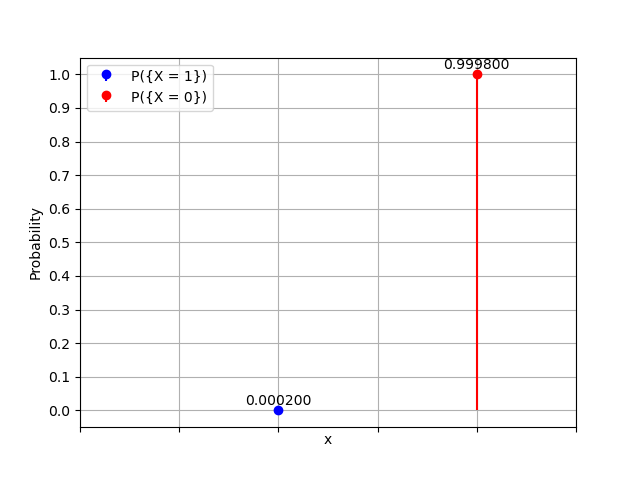
\includegraphics[width=0.5\linewidth]{figs/pmf.png}
    \caption{PMF of the Random Variable}
    \label{fig:enter-label}
\end{figure}

\begin{figure}
    \centering
    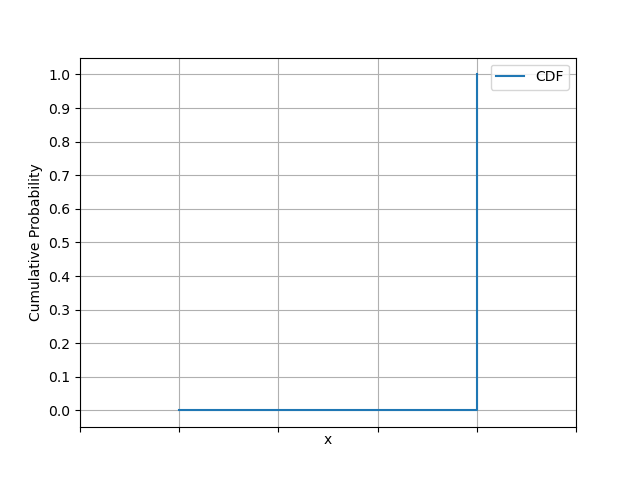
\includegraphics[width=0.5\linewidth]{figs/cdf.png}
    \caption{CDF of the Random Variable}
    \label{fig:enter-label}
\end{figure}
\end{document}i
